\documentclass{beamer}
%\documentclass{powerdot}
%\documentclass{slides}[14pt]
%\pagestyle{empty}
%\normalsize
\usepackage{amsmath}
\usepackage{amssymb}
\usepackage{amscd}
% \usepackage{moreverb}
\usepackage{graphicx}
% \usepackage[all]{xy}
% \usepackage{beamerthemesplit}


\input macros			   %% loan from John Gibson's snowbird 07 talk
% \input ../../inputs/defsThesis     %% all Vaggelis edits: \renewcommand, etc

% Setup appearance:

\usetheme{Darmstadt}
\usefonttheme[onlylarge]{structurebold}
\setbeamerfont*{frametitle}{size=\normalsize,series=\bfseries}
\setbeamertemplate{navigation symbols}{}

% Standard packages

\usepackage[english]{babel}
\usepackage[latin1]{inputenc}
\usepackage{times}
\usepackage[T1]{fontenc}


% % Setup TikZ
% 
% \usepackage{tikz}
% \usetikzlibrary{arrows}
% \tikzstyle{block}=[draw opacity=0.7,line width=1.4cm]

\title{Recurrent spatio-temporal structures in presence of continuous symmetries}
\author{Evangelos Siminos}
\institute{Center for Nonlinear Science\\ School of Physics\\ Georgia Institute of Technology}
\date{March 23, 2009}

\begin{document}

\begin{frame}
  \titlepage
\end{frame}

\begin{frame}{Outline}
  \tableofcontents
\end{frame}

\section{Introduction}

\subsection{Dynamicist's vision of Turbulence}

\begin{frame}{Turbulence}
 	
\end{frame}

\begin{frame}{PO's and beyond}
\end{frame}

\subsection{This thesis}

\begin{frame}{Symmetry}
\end{frame}

\begin{frame}{\KSe}
 
\end{frame}

\section{(De-)symmetrization}

\subsection{$G$-background}

\begin{frame}{Symmetry}

\begin{columns}
 \column{0.6\textwidth}
	\begin{itemize}
		\item A set has a symmetry if it is invariant under a transformation.
		\item Symmetry transformations form groups acting on \Rls{n}.
		\item Here we consider subgroups of \On{n}.
	\end{itemize}
 \column{0.3\textwidth}
	\begin{exampleblock}{Equilateral triangle}
	 	\begin{center}
			\includegraphics[width=.7\textwidth]{../../figs/D3triangle}
		\end{center}
	\Dn{3} acting on \Clx{} by
	\[
	\begin{split}	
  		\Drot z &= e^{i\frac{2\pi}{3}} z\,,\\
  		\Refl z  &= \conj{z}\,.
 	\end{split}
	\]
	\end{exampleblock}
\end{columns}

\end{frame}

\begin{frame}{Isotropy subgroups}

Not all points have the same symmetry:
\begin{columns}
  \column{0.7\textwidth}
	\begin{block}{Group orbit of $x$}
	\[
	\Gamma x = \{\gamma x: \gamma\in\Gamma\}\,.
	\]
	\end{block}
 	\begin{block}{Isotropy subgroup}
 	\[
 	\stab{x}=\{\gamma\in\Gamma:\gamma x=x\}\,.
 	\]
 	\end{block}
  \column{0.3\textwidth}
 	\begin{exampleblock}{Equilateral triangle}
 	 	\begin{center}
 			\includegraphics[width=.7\textwidth]{../../figs/D3triangle}
 		\end{center}
	$\Gamma x_A=\{x_B,x_C\}$
 	$\stab{x_A}=\{e,\Refl\}\cong\Dn{1}$
 	\end{exampleblock}
\end{columns}

\end{frame}

\frame{Fixed point subspaces}


\begin{frame}{Symmetry in differential equations}

\begin{block}{}
 We call a group element $\gamma\in\On{n}$ a symmetry of
\[
	\dot{x} = \vf(x,\lambda)\,,
	\label{eq:difeq} 
\]  
if for every solution $x(t)$, $\gamma x(t)$ is also a solution.
\end{block}

\end{frame}

\subsection{Desymmetrization of \CLe}

\begin{frame}{\CLe}
  \begin{columns}[t]
    \column{.4\textwidth}
    \begin{exampleblock}{\CLe}
      	\[
		\begin{split}
			\dot{x} &=-\sigma x+ \sigma y \,,\\
			\dot{y} &=(r-z)x-a y \,,\\
			\dot{z} &= \frac{1}{2}\left(x y^*+x^*y\right)-b z\,.
		\end{split}
	\]
    \end{exampleblock}
     \begin{block}{ }
       $x,y\in\Clx{}$, $z\in\Rls{}$ parameters $\sigma,\,b\in\Rls{}$, $r=r_1+i\, r_2$, $a=1-i\, e$, $r_1,\,r_2,\,e\in\Rls{}$.
    \end{block}

    \column{.5\textwidth}
    \begin{exampleblock}{Equivariant under}
	$SO(2)$ acting by
      	\[
	\begin{split}
 		\Rot{\theta} (x,y,z) &= (e^{i\theta} x, e^{i\theta} y, z)\,, \\
			\theta	& \in[0,2\pi)\,.
	\end{split}
	\]
    \end{exampleblock}
    \begin{exampleblock}{Physics}
	For $r_2=0$ appears as a truncation of Maxwell-Bloch equation
	that describes ring laser with detuning proportional to $e$.
    \end{exampleblock}

  \end{columns}
\end{frame}

\begin{frame}
  \begin{columns}[t]
     \column{.6\textwidth}
	\begin{block}{}
	\begin{center}
		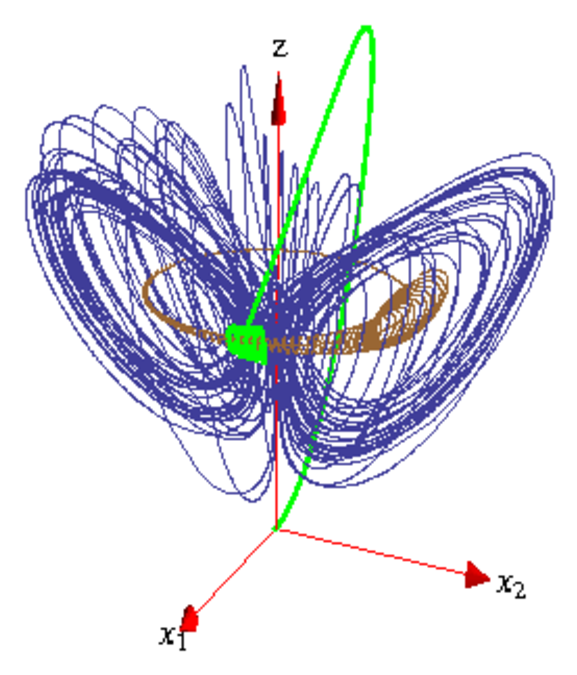
\includegraphics[width=.7\textwidth]{../../figs/CLE.eps}
	\end{center}
	\end{block}
     \column{.4\textwidth}
	\begin{block}{ }
	 ${r_1=28,}\, {b=8/3,}\,$ ${\sigma=10,}\, {a=1,}\,$ ${e=1/10,}\, {r_2=0}$
	\end{block}
	\begin{block}{ }
	  $E_0$: saddle\\
	  $Q_1$: relative equilibrium\\ 
	  $01$:  relative periodic orbit $T_{01}=1.542,\, \theta_{01}=2.953$
	\end{block}
   \end{columns}
\end{frame}


\begin{frame}{\CLe\ reduction by invariant polynomials}
\end{frame}

\begin{frame}{\CLe\ reduction by local invariants}
\end{frame}

\begin{frame}{\CLe\ reduction by local invariants II}
\end{frame}

\begin{frame}{\CLe\ reduction by double section}
\end{frame}


\section[\KSe]{\KS, $L=22$, phase space }

\subsection{\KSe}

\begin{frame}{\KSe}
\[
  u_t = F(u) = -{\textstyle\frac{1}{2}}(u^2)_x-u_{xx}-u_{xxxx}
    \,,\qquad   x \in [-L/2,L/2]
    \,,
\]
Appears in study of many extended systems including
\begin{itemize}
 \item reaction-diffusion systems
 \item combustion problems (flame fronts)
 \item thin falling films
 \item and more\ldots
\end{itemize}


Impose periodic boundary conditions:
\[
 u(x,t) = u(x+L,t)
\]
\end{frame}

\begin{frame}{Symmetries of \KSe}

\begin{itemize}
 \item Galilean invariance: if $u(x,t)$ is a solution, then $u(x-ct,t)-c$, with $c$ an arbitrary constant
	speed, is also a solution.
	\begin{itemize}
		\item The mean $u_0=\int_{-L/2}^{L/2} u dx$ is a constant of the motion. \\
		\item Setting $u_0=0$ corresponds to choosing $c=0$ therefore eliminating Galilean invariance.
	\end{itemize}
 \item Equivariant under $\On{2}$:
\[
	\Shift_{\shift/L}\, u(x,t) = u(x+\shift,t)\,,\qquad \shift\in\left[-L/2,L/2\right]\,,
\]

\[
    \Refl \, u(x) = -u(-x)
\,.
\]
\end{itemize}
\end{frame}

\begin{frame}{Fourier space}
Use
\[
  u(x,t)=\sum_{k=-\infty}^{+\infty} a_k (t) e^{ i q_k x }
\]
where
\[
 q_k = 2\pi\,k/L.
\]
Get
\[
 \dot{a}_k
     = ( q_k^2 - q_k^4 )\, a_k
    - i \frac{q_k}{2} \sum_{m=-\infty}^{+\infty} a_m a_{k-m}\,,
\]
with $a_{k}=a^\ast_{-k}$ since $u(x,t)$ is real.

Truncate to finite order $N$.
\end{frame}

\begin{frame}{Symmetry in Fourier space}

Symmetry acts as
\[
  \Shift_{\shift/L}\, a = \mathbf{g}(\shift) \, a \,,
  \label{eq:shiftF}
\]
\[
   \Refl \, a = -a^\ast
\]
where $\mathbf{g}(\shift) = \mathrm{diag}( e^{i q_k\, \shift} )$.

\end{frame}




\subsection{Antisymmetric subspace}

\subsection{Full space}

\section*{Summary}
\begin{frame}
\frametitle<presentation>{Summary}

In summary

\end{frame}


\end{document}
